


Very roughly speaking, a principal fibre bundle is a bundle whose typical fibre is a Lie group. Principal fibre bundles are so immensely important because they allow us to understand any fibre bundle with fibre $F$ on which a Lie group $G$ acts. These are then called associated fibre bundles, and will be discussed later on.

\subsection{Lie group actions on a manifold}

\bd
Let $(G,\bullet)$ be a Lie group and let $M$ be a smooth manifold. A smooth map
\bi{rrCl}
\lacts \cl & G\times M & \to & M\\
& (g,p) & \mapsto & g \lacts p
\ei
satisfying
\ben[label=\roman*)]
\item $\forall \, p \in M :\ e\lacts p = p$;
\item $\forall \, g_1,g_2\in G : \forall \, p\in M : \ (g_1\bullet g_2) \lacts p = g_1 \lacts (g_2 \lacts p)$,
\een
is called a \emph{left Lie group action}\index{Lie group action}\index{group action}, or \emph{left $G$-action}, on $M$. 
\ed
\bd
A manifold equipped with a left $G$-action is called a \emph{left $G$-manifold}.
\ed
\br
Note that in the above definition, the smooth structures on $G$ and $M$ were only used in the requirement that $\lacts$ be smooth. By dropping this condition, we obtain the usual definition of a group action on a set. Some of the definitions that we will soon give for Lie groups and smooth manifolds, such as those of orbits and stabilisers, also have clear analogues to the case of bare groups and sets.
\er

\be
Let $G$ be a Lie group and let $R\cl G \to \GL(V)$ be a representation of $G$ on a vector space $V$. Define a map
\bi{rrCl}
\lacts \cl & G \times V & \to & V\\
& (g,v) & \mapsto & g\lacts v := R(g)v.
\ei
We easily check that $e\lacts v := R(e)v = \id_V v = v$ and
\bi{rCl}
(g_1\bullet g_2) \lacts v & := & R(g_1\bullet g_2)v\\
& = & (R(g_1)\circ R(g_2))v\\
& = & R(g_1)( R(g_2)v)\\
& = & g_1 \lacts (g_2 \lacts v),
\ei
for any $v\in V$ and any $g_1,g_2\in G$. Moreover, if we equip $V$ with the usual smooth structure, the map $\lacts$ is smooth and hence a Lie group action on $V$. It follows that representations of Lie groups are just a special case of left Lie group actions. We can therefore think of left $G$-actions as generalised representations of $G$ on some manifold.
\ee

\bd
Similarly, a \emph{right $G$-action} on $M$ is a smooth map
\bi{rrCl}
\racts \cl & M\times G & \to & M\\
& (p,g) & \mapsto & p \racts g
\ei
satisfying
\ben[label=\roman*)]
\item $\forall \, p \in M :\ p\racts g = p$;
\item $\forall \, g_1,g_2\in G : \forall \, p\in M : \ p \racts (g_1\bullet g_2) = (p \racts g_1) \racts g_2$.
\een
\ed

\bp
Let $\lacts$ be a left $G$-action on $M$. Then
\bi{rrCl}
\racts \cl & M\times G & \to & M\\
& (p,g) & \mapsto & p \racts g := g^{-1} \lacts p
\ei
is a right $G$-action on $M$.
\ep
\bq
First note that $\racts$ is smooth since it is a composition of $\lacts$ and the inverse map on $G$, which are both smooth. We have $p\racts e := e \lacts p = p$ and
\bi{rCl}
p \racts  (g_1\bullet g_2) & := & (g_1\bullet g_2)^{-1} \lacts p\\
& = & (g_2^{-1}\bullet g_1^{-1}) \lacts p\\
& = & g_2^{-1} \lacts (g_1^{-1} \lacts p)\\
& = & g_2^{-1} \lacts (p \racts g_1)\\
& = & (p \vartriangleleft g_1) \vartriangleleft g_2,
\ei
for all $p\in M$ and $g_1,g_2\in G$, and hence $\racts$ is a right $G$-action.
\eq

\br
Since for each $g\in G$ we also have $g^{-1}\in G$, if we need \emph{some} action of $G$ on $M$, then a left action is just as good as a right action. Only later, within the context of principal and associated fibre bundles, we will attach separate ``meanings'' to left and right actions. Some of the next definitions and results will only be given in terms of left actions, but they obviously apply to right actions as well.
\er

\br
Recall that if we have a basis $e_1,\ldots,e_{\dim M}$ of $T_pM$ and $X^1,\ldots,X^{\dim M}$ are the components of some $X\in T_pM$ in this basis, then under a change of basis
\bse
\widetilde e_a = A^b_{\phantom{b}a}e_b,
\ese
we have $X=\widetilde X^a \widetilde e_a$, where
\bse
\widetilde X^a = (A^{-1})^a_{\phantom{a}b}X^b.
\ese
Once expressed in terms of principal and associated fibre bundles, we will see that the ``recipe'' of labelling the basis by lower indices and the vector components by upper indices, as well as their transformation law, can be understood as a right action of $\GL(\dim M, \R)$ on the basis and a left action of the same $\GL(\dim M, \R)$ on the components.
\er

\bd
Let $G,H$ be Lie groups, let $\rho\cl G\to H$ be a Lie group homomorphism and let
\bi{l}
\lacts \cl G \times M \to M,\\
\blacktriangleright \cl H \times N \to N
\ei
be left actions of $G$ and $H$ on some smooth manifolds $M$ and $N$, respectively. Then, a smooth map $f\cl M\to N$ is said to be \emph{$\rho$-equivariant} if the diagram
\bse
\begin{tikzcd}
G\times M \ar[dd,"\lacts"'] \ar[rr,"\rho\times f"]&& H\times N \ar[dd,"\blacktriangleright"]\\
&&\\
M \ar[rr,"f"] && N
\end{tikzcd}
\ese
where $(\rho\times f)(g,p) := (\rho(g),f(p))\in H\times N$, commutes. Equivalently,
\bse
\forall \, g \in G : \forall \, p \in M : \ f(g\lacts p) = \rho(g)\blacktriangleright f(p).
\ese
\ed

In other words, if $\rho\cl G \to H$ is a Lie group homomorphism, then the $\rho$-equivariant maps are the ``action-preserving'' maps between the $G$-manifold $M$ and the $H$-manifold $N$.

\br
Note that by setting $\rho = \id_G$ or $f=\id_M$, the notion of $f$ being $\rho$-equivariant reduces to what we might call a homomorphism of $G$-manifolds in the former case, and a homomorphism of left actions on $M$ in the latter.
\er

\bd
Let $\lacts \cl G \times M \to M$ be a left $G$-action. For each $p\in M$, we define the \emph{orbit}\index{orbit} of $p$ as the set
\bse
G_p :=\{q\in M\mid \exists \, g\in G : q = g\lacts p\}.
\ese
\ed

Alternatively, the orbit of $p$ is the image of $G$ under the map $( {}-\lacts p)$. It consists of all the points in $M$ that can be reached from $p$ by successive applications of the action $\lacts$.

\be
Consider the action induced by representation of $\SO(2,\R)$ as rotation matrices in $\End(\R^2)$. The orbit of any $p\in\R^2$ is the circle of radius $|p|$ centred at the origin.
\begin{center}
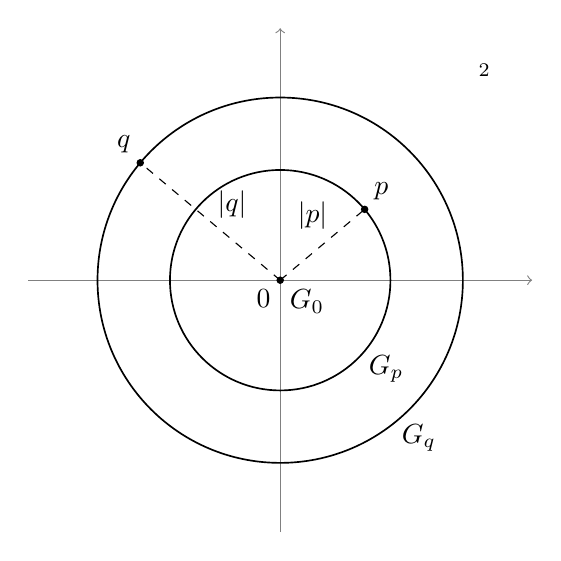
\begin{tikzpicture}[scale=0.8]
\draw[gray,->] (0,-4) -- (0,4);
\draw[gray,->] (-4,0) -- (4,0);
\draw (3.25,3.25) node {$\R^2$};
\draw[dashed] (0,0) -- (1.75*cos 40 , 1.75*sin 40) node[above right] {$p$};
\draw[fill] (1.75*cos 40 , 1.75*sin 40) circle[radius=0.05];
\draw (1.75*cos -40 , 1.75*sin -40) node[below right=-2pt] {$G_p$};
\draw (-0.1+0.8*cos 40 , 0.8*sin 40) node[above=3pt] {$|p|$};
\draw[dashed] (0,0) -- (2.9*cos 140 , 2.9*sin 140) node[above left] {$q$};
\draw[fill] (2.9*cos 140 , 2.9*sin 140) circle[radius=0.05];
\draw (2.9*cos -50 , 2.9*sin -50) node[below right=-2pt] {$G_q$};
\draw(1*cos 140 , 1*sin 140) node[above=4pt ] {$|q|$};
\draw[semithick] (0,0) circle [radius=1.75];
\draw[semithick] (0,0) circle [radius=2.9];
\draw[fill] (0,0) circle [radius=0.05] node[below right] {$G_0$};
\draw(0,0)  node[below left] {$0$};
\end{tikzpicture}
\end{center}
\ee

It should be intuitively clear from the definition that the orbits of two points are either disjoint or coincide. In fact, we have the following.

\bp
Let $\lacts \cl G\times M \to M$ be an action on $M$. Define a relation on $M$
\bse
p\sim q \ :\Leftrightarrow \ \exists \, g \in G : q = g \lacts p.
\ese
Then $\sim$ is an equivalence relation on $M$.
\ep

\bq
Let $p,q,r\in M$. We have
\begin{enumerate}[label=\roman*)]
\item $p\sim p$ since $p = e \lacts p$;
\item $p\sim q \Rightarrow q\sim p$ since, if $q =g \lacts p$, then
\bse
p = e \lacts p = (g^{-1}\bullet g) \lacts p = g^{-1}\lacts( g \lacts p)= g^{-1}\lacts q; 
\ese
\item $(p\sim q$ and $q\sim r) \Rightarrow p\sim r$ since, if $q =g_1 \lacts p$ and $r =g_2 \lacts q$, then
\bse
r = g_2 \lacts (g_1 \lacts p) = (g_1\bullet g_2)\lacts p.
\ese
\end{enumerate}
Therefore, $\sim$ is an equivalence relation on $M$.
\eq
The equivalence classes of $\sim$ are, by definition, the orbits.
\bd
Let $\lacts\cl G\times M\to M$ be an action on $M$. The \emph{orbit space} of $M$ is
\bse
M/G := M/\!\sim \,= \{G_p \mid p\in M\}.
\ese
\ed
\be
The orbit space of our previous $\SO(2,\R)$-action on $\R^2$ is the partition of $\R^2$ into concentric circles centred at the origin, plus the origin itself.
\ee
\bd
Let $\lacts\cl G\times M\to M$ be a $G$-action on $M$. The \emph{stabiliser}\index{stabiliser} of $p\in M$ is
\bse
S_p:=\{g\in G\mid g\lacts p = p\}.
\ese
\ed
Note that for each $p\in M$, the stabiliser $S_p$ is a subgroup of $G$.
\be
In our $\SO(2,\R)$ example, we have $S_p=\{\id_{\R^2}\}$ for $p\neq 0$ and $S_0=\SO(2,\R)$.
\ee
\bd
A left $G$-action $\lacts\cl G\times M\to M$ is said to be
\ben[label=\roman*)]
\item \emph{free} if for all $p\in M$, we have $S_p=\{e\}$;
\item \emph{transitive} if for all $p,q\in M$, there exists $g\in G$ such that $p=g\lacts p$.
\een
\ed

\be
The action $\lacts\cl G\times V \to V$ induced by a representation $R\cl G\to \GL(V)$ is never free since we always have $S_0=G$.
\ee

\be
Consider the action $\lacts\cl \mathrm{T}(n)\times \R^n\to \R^n$ of the $n$-dimensional translation group $\mathrm{T}(n)$ on $\R^n$. We have, rather trivially, $\mathrm{T}(n)_p=\R^n$ for every $p\in \R^n$.It is also easy to show that this action is free and transitive. 
\ee

\bp
Let $\lacts\cl G \times M \to M$ be a free action. Then
\bse
g_1 \lacts p = g_2 \lacts p \quad \Leftrightarrow \quad g_1 = g_2.
\ese
\ep
\bq
The $(\Leftarrow)$ direction is obvious. Suppose that there exist $p\in M$ and $g_1,g_2\in G$ such that $g_1 \lacts p = g_2 \lacts p$. Then
\bi{rCl}
g_1 \lacts p = g_2 \lacts p  &\quad  \Leftrightarrow \quad & g_2^{-1} \lacts (g_1 \lacts p) = g_2^{-1} \lacts(g_2 \lacts p)\\
& \Leftrightarrow & (g_2^{-1} \bullet g_1) \lacts p = (g_2^{-1}\bullet g_2) \lacts p\\
& \Leftrightarrow & (g_2^{-1}\bullet g_1)  \lacts p = (e\lacts p)\\
& \Leftrightarrow & (g_2^{-1}\bullet g_1)  \lacts p = p.
\ei
Hence $g_2^{-1}\bullet g_1\in S_p$, but since $\lacts$ is free we have $S_p=\{e\}$, and thus $g_1=g_2$.
\eq

\bp
If $\lacts\cl G \times M \to M$ is a free action, then
\bse
\forall \, p \in G :\ G_p \cong_{\mathrm{diff}} G.
\ese
\ep

\be
Define $\lacts\cl \SO(2,\R)\times \R^2\sm\{0\}\to \R^2\sm\{0\}$ to coincide with the action induced by the representation of $\SO(2,\R^2)$ on $\R^2$ for each non-zero point of $\R^2$. Then this action is free, since we have $S_p=\{\id_{\R^2}\}$ for $p\neq 0$, and the previous proposition implies
\bse
\forall \, p\in \R^2\sm\{0\} : \ \SO(2,\R)_p \cong_{\mathrm{diff}} \SO(2,\R) \cong_{\mathrm{diff}} S^1.
\ese
\ee


\subsection{Principal fibre bundles}

This is a good time to review our earlier section on bundles. We can specialize our definition of bundle to define a \emph{smooth bundle}, which is just a bundle $(E,\pi,M)$ where $E$ and $M$ are smooth manifolds and the projection $\pi\cl E\to M$ is smooth. Two smooth bundles $(E,\pi,M)$ and $(E',\pi',M')$ are isomorphic if there exist diffeomorphisms $u,f$ such that the following diagram commutes
\bse
\begin{tikzcd}
E \ar[dd,"\pi"'] \ar[rr,"u"] && E' \ar[dd,"\pi'"]\\
&&\\
M\ar[rr,"f"] && M'
\end{tikzcd}
\ese

\bd
Let $G$ be a Lie group. A smooth bundle $(E,\pi,M)$ is called a \emph{principal $G$-bundle}\index{principal bundle} if $E$ is equipped with a free right $G$-action and
\bse
\begin{tikzcd}
E \ar[d,"\pi"'] \\
M 
\end{tikzcd}
\ \ \cong_{\mathrm{bdl}}
\begin{tikzcd}
  E \ar[d,"\rho"]\\
  E/G
\end{tikzcd}
\ese
where $\rho$ is the quotient map, defined by sending each $p\in E$ to its equivalence class (i.e.\ orbit) in the orbit space $E/G$.
\ed
Observe that since the right action of $G$ on $E$ is free, for each $p\in E$ we have
\bse
\preim_\rho(G_p) = G_p \cong_{\mathrm{diff}} G.
\ese
We said at beginning that, roughly speaking, a principal bundle is a bundle whose fibre at each point is a Lie group. Note that the formal definition is that a principal $G$-bundle is a bundle which is isomorphic to a bundle whose fibres are the orbits under the right action of $G$, which are themselves isomorphic to $G$ since the action is free.

\br
A slight generalisation would be to consider smooth bundles $E\xrightarrow{\,\pi\,}M$ where $E$ is equipped with a right $G$-action which is free and transitive on each fibre of $E\xrightarrow{\,\pi\,}M$. The isomorphism in our definition enforces the fibre-wise transitivity since $G$ acts transitively on each $G_p$ by the definition of orbit.
\er

\be
\ben[label=\alph*)]
\item Let $M$ be a smooth manifold. Consider the space
\bse
L_pM := \{(e_1,\ldots,e_{\dim M})\mid e_1,\ldots,e_{\dim M} \text{ is a basis of }T_pM\} \cong_{\mathrm{vec}} \GL(\dim M,\R).
\ese
We know from linear algebra that the bases of a vector space are related to each other by invertible linear transformations. Hence, we have 
\bse
L_pM \cong_{\mathrm{vec}} \GL(\dim M,\R).
\ese
We define the frame bundle of $M$ as
\bse
LM := \coprod_{p\in M} L_pM
\ese
with the obvious projection map $\pi\cl LM \to M$ sending each basis $(e_1,\ldots,e_{\dim M})$ to the unique point $p\in M$ such that $(e_1,\ldots,e_{\dim M})$ is a basis of $T_pM$.
By proceeding similarly to the case of the tangent bundle, we can equip $LM$ with a smooth structure inherited from that of $M$. We then find
\bse
\dim LM = \dim M + \dim T_pM = \dim M + (\dim M)^2.
\ese
\item We would now like to make $LM \xrightarrow{\,\pi\,}M$ into a principal $\GL(\dim M,\R)$-bundle. We define a right $\GL(\dim M,\R)$-action on $LM$ by
\bse
(e_1,\ldots,e_{\dim M}) \racts g := (g^a_{\phantom{a}1}e_a,\ldots,g^a_{\phantom{a}\dim M}e_a),
\ese
where $g^a_{\phantom{a}b}$ are the components of the endomorphism $g\in \GL(\dim M, \R)$ with respect to the standard basis on $\R^n$. Note that if $(e_1,\ldots,e_{\dim M})\in L_pM$, we must also have $(e_1,\ldots,e_{\dim M}) \racts g\in L_pM$. This action is free since
\bse
(e_1,\ldots,e_{\dim M}) \racts g = (e_1,\ldots,e_{\dim M})  \Leftrightarrow  (g^a_{\phantom{a}1}e_a,\ldots,g^a_{\phantom{a}\dim M}e_a)= (e_1,\ldots,e_{\dim M}) 
\ese
and hence, by linear independence, $g^a_{\phantom{a}b}=\delta^a_b$, so $g=\id_{\R^n}$. Note that since all bases of each $T_pM$ are related by some $g\in \GL(\dim M,\R)$, $\racts$ is also fibre-wise transitive. 
\item We now have to show that
\bse
\begin{tikzcd}
LM \ar[d,"\pi"'] \\
M 
\end{tikzcd}
\ \ \cong_{\mathrm{bdl}}
\begin{tikzcd}
  LM \ar[d,"\rho"]\\
  LM \big/ \GL(\dim M,\R)
\end{tikzcd}
\ese
i.e.\ that there exist smooth maps $u$ and $f$ such that the diagram
\bse
\begin{tikzcd}
LM \ar[rr,shift left,"u"] \ar[dd,"\pi"']&& LM \ar[ll,shift left,"u^{-1}"]\ar[dd,"\rho"]\\
&&\\
M \ar[rr,shift left,"f"]&&  LM \big/ \GL(\dim M,\R)\ar[ll,shift left,"f^{-1}"]
\end{tikzcd}
\ese
commutes. We can simply choose $u=u^{-1}=\id_{LM}$, while we define $f$ as
\bi{rrCl}
f \cl & M & \to &  LM\big/ \GL(\dim M,\R)\\[2pt]
& p & \mapsto & \GL(\dim M,\R)_{(e_1,\ldots,e_{\dim M})},
\ei
where $(e_1,\ldots,e_{\dim M})$ is some basis of $T_pM$, i.e.\ $(e_1,\ldots,e_{\dim M})\in \preim_\pi(\{p\})$. Note that $f$ is well-defined since every basis of $T_pM$ gives rise to the same orbit in the orbit space $LM\big/\GL(\dim M,\R)$. Moreover, it is injective since
\bse
f(p)=f(p')\ \Leftrightarrow \ \GL(\dim M,\R)_{(e_1,\ldots,e_{\dim M})} = \GL(\dim M,\R)_{(e'_1,\ldots,e'_{\dim M})},
\ese
which is true only if $(e_1,\ldots,e_{\dim M})$ and $(e'_1,\ldots,e'_{\dim M})$ are basis of the same tangent space, so $p=p'$. It is clearly surjective since every orbit in $LM\big/ \GL(\dim M,\R)$ is the orbit of some basis of some tangent space $T_pM$ at some point $p\in M$. The inverse map is given explicitly by
\bi{rrCl}
f^{-1} \cl & LM\big/ \GL(\dim M,\R) & \to & M \\[2pt]
& \GL(\dim M,\R)_{(e_1,\ldots,e_{\dim M})} & \mapsto & \pi((e_1,\ldots,e_{\dim M})).
\ei
Finally, we have
\bse
(\rho\circ\id_{LM})(e_1,\ldots,e_{\dim M}) = \GL(\dim M,\R)_{(e_1,\ldots,e_{\dim M})} = (f\circ \pi)(e_1,\ldots,e_{\dim M})
\ese
and thus $LM\xrightarrow{\,\pi\,}M$ is a principal $G$-bundle, called the \emph{frame bundle}\index{frame bundle} of $M$.
\een
\ee

\br
A note to the careful reader. As we have just done in the previous example, in the following we will sometimes simply assume that certain maps are smooth, instead of rigorously proving it. 
\er

\subsection{Principal bundle morphisms}

Recall that a bundle morphism (also called simply a bundle map) between two bundles $(E,\pi,M)$ and $(E',\pi',M')$ is a pair of maps $(u,f)$ such that the diagram
\bse
\begin{tikzcd}
E \ar[dd,"\pi"'] \ar[rr,"u"] && E' \ar[dd,"\pi'"]\\
&&\\
M\ar[rr,"f"] && M'
\end{tikzcd}
\ese
commutes, that is, $f\circ \pi = \pi' \circ u$.
\bd
Let $(P,\pi,M)$ and $(Q,\pi',N)$ be principal $G$-bundles. A \emph{principal bundle morphism} from $(P,\pi,M)$ to $(Q,\pi',N)$ is a pair of smooth maps $(u,f)$ such that the diagram
\bse
\begin{tikzcd}
P \ar[rr,"u"]&& Q \\
&&\\
P \ar[uu,"{}\racts G"] \ar[dd,"\pi"'] \ar[rr,"u"] && Q\ar[uu,"{}\blacktriangleleft G"'] \ar[dd,"\pi'"]\\
&&\\
M\ar[rr,"f"] && N
\end{tikzcd}
\ese
commutes, that is for all $p\in P$ and $g\in G$, we have
\bi{rCl}
(f\circ \pi)(p)  & = & (\pi'\circ u)(p)\\
u(p\racts g) & = & u(p)\blacktriangleleft g.
\ei
\ed
Note that $P\xrightarrow{\quad \racts G \quad } P$ is a shorthand for the inclusion of $P$ into the product $P\times G$ followed by the right action $\racts$, i.e.\
\bse
\begin{tikzcd}
P \ar[rr,"\racts G"] && P
\end{tikzcd}
\ \quad =\quad \ 
\begin{tikzcd}
P \ar[rr,"i_1"] && P\times G \ar[rr,"\racts"] && P
\end{tikzcd}
\ese
and similarly for $Q\xrightarrow{\quad \blacktriangleleft G \quad } Q$.

\bd
A principal bundle morphism between two principal $G$-bundles is an \emph{isomorphism} (or \emph{diffeomorphism}) \emph{of principal bundles} if it is also a bundle isomorphism.
\ed

\br
Note that the passage from principal bundle morphism to principal bundle isomorphism does not require any extra condition involving the Lie group $G$. We will soon see that this is because the two bundles are both principal $G$-bundles. We can further generalise the notion of principal bundle morphism as follows.
\er

\bd
Let $(P,\pi,M)$ be a principal $G$-bundle, let $(Q,\pi',N)$ be a principal $H$-bundle, and let $\rho\cl G \to H$ be a Lie group homomorphism. A \emph{principal bundle morphism}\index{principal bundle morphism} from $(P,\pi,M)$ to $(Q,\pi',N)$ is a pair of smooth maps $(u,f)$ such that the diagram
\bse
\begin{tikzcd}
P \ar[rr,"u"]&& Q \\
&&\\
P\times G\ar[uu,"{}\racts "]  \ar[rr,"u\times \rho"]&& Q\times H \ar[uu,"{}\blacktriangleleft"'] \\
&&\\
P \ar[uu,"i_1"] \ar[dd,"\pi"'] \ar[rr,"u"] && Q\ar[uu,"i_1"'] \ar[dd,"\pi'"]\\
&&\\
M\ar[rr,"f"] && N
\end{tikzcd}
\ese
commutes, that is $f \circ \pi=\pi'\circ u $ and $u$ is a $\rho$-equivariant map
\bi{rCl}
\forall \, p\in P : \forall \, g \in G : \ u(p\racts g) & = & u(p)\blacktriangleleft \rho(g).
\ei
\ed

\bd
A principal bundle morphism between principal $G$-bundle and a principal $H$-bundle is an \emph{isomorphism} (or \emph{diffeomorphism}) \emph{of principal bundles}\index{isomorphism!of principal bundles} if it is also a bundle isomorphism and $\rho$ is a Lie group isomorphism.
\ed

\bl
Let $(P,\pi,M)$ and $(Q,\pi',M)$ be principal $G$-bundles over the same base manifold $M$. Then, any $u\cl P \to Q$ such that $(u,\id_M)$ is a principal bundle morphism is necessarily a diffeomorphism.
\bse
\begin{tikzcd}
P \ar[rr,"u"]&& Q \\
&&\\
P \ar[uu,"\racts G"] \ar[ddr,"\pi"'] \ar[rr,"u"] && Q\ar[uu,"\blacktriangleleft G"'] \ar[ddl,"\pi'"]\\
&&\\
 &M& 
\end{tikzcd}
\ese
\el

\bq
We already know that $u$ is smooth since $(u,\id_M)$ is assumed to be a principal bundle morphism. It remains to check that $u$ is bijective and its inverse is also smooth.
\ben[label=\roman*)]
\item Let $p_1,p_2\in P$ be such that $u(p_1)=u(p_2)$. Then
\bse
\pi(p_1) = \pi'(u(p_1)) = \pi'(u(p_2)) = \pi(p_2),
\ese
that is, $p_1$ and $p_2$ belong to the same fibre. As the action of $G$ on $P$ is fibre-wise transitive, there is a unique $g\in G$ such that $p_1 = p_2\racts g$. Then
\bse
u(p_1)  = u(p_2\racts g)  = u(p_2) \blacktriangleleft g = u(p_1) \blacktriangleleft g,
\ese
so $g\in S_{u(p_1)}$, but since $\blacktriangleleft$ is free, we have $g=e$ and thus
\bse
p_1 = p_2\racts e = p_2.
\ese
Therefore $u$ is injective.
\item Let $q\in Q$. Choose some $p\in \preim_\pi(\pi'(q))$. Then, we have
\bse
\pi'(u(p)) = \pi(p) = \pi'(q)
\ese
so that $u(p)$ and $q$ belong to the same fibre. Hence, there is a unique $g\in G$ such that $q = u(p)\blacktriangleleft g$. We thus have
\bse
q = u(p)\blacktriangleleft g = u(p\racts g)
\ese
and since $p\racts g\in P$, the map $u$ is surjective. 
\een
Hence, $u$ is a diffeomorphism.
\eq


\bd
A principal $G$-bundle $(P,\pi,M)$ if it is called \emph{trivial} if it is isomorphic as a principal $G$-bundle to the principal $G$-bundle $(M\times G,\pi_1,M)$ where $\pi_1$ is the projection onto the first component and the action is defined as
\bi{rrCl}
\blacktriangleleft \cl & (M\times G) \times G & \to &M\times G\\
& ((p,g),g') & \mapsto & (p,g)\blacktriangleleft g' := (p,g\bullet g').
\ei
\ed
By the previous lemma, a principal $G$-bundle $(P,\pi,M)$ is trivial if there exists a smooth map $u\cl P\to M\times G$ such that the following diagram commutes.
\bse
\begin{tikzcd}
P \ar[rr,"u"]&& M\times G \\
&&\\
P \ar[uu,"{}\racts G"] \ar[ddr,"\pi"'] \ar[rr,"u"] && M\times G\ar[uu,"{}\blacktriangleleft G"'] \ar[ddl,"\pi_1"]\\
&&\\
& M & 
\end{tikzcd}
\ese

The following result provides a necessary and sufficient criterion for when a principal bundle is trivial. Note that while we have used the lower case letter $p$ almost exclusively to denote points of the base manifold $M$, in the next proof we will use it to denote points of the total space $P$ instead.

\begin{theorem}
A principal $G$-bundle $(P,\pi,M)$ is trivial if, and only if, there exists a smooth section $\sigma\in\Gamma(P)$, that is, a smooth $\sigma \cl M \to P$ such that $\pi\circ \sigma = \id_M$.
\end{theorem}

\bq
\begin{itemize}
\item[$(\Rightarrow)$] Suppose that $(P,\pi,M)$ is trivial. Then there exists a diffeomorphism $u\cl P \to M\times G$ which make the following diagram commute
\bse
\begin{tikzcd}
P && \\
&&\\
P \ar[uu,"{}\racts G"] \ar[ddr,"\pi"']  && M \ar[ll,"u^{-1}"'] \times G\ar[ddl,"\pi_1"]\\
&&\\
& M & 
\end{tikzcd}
\ese
We can define
\bi{rrCl}
\sigma \cl & M & \to & P\\
& m & \mapsto & u^{-1}(m,e),
\ei
where $e$ is the identity of $G$. Then $\sigma$ is smooth since it is the composition of $u^{-1}$ with the map $p\mapsto (p,e)$, which are both smooth. We also have
\bse
(\pi\circ\sigma)(pm=\pi( u^{-1}(m,e)) = \pi_1 (m,e) = m,
\ese
for all $m\in M$, hence $\pi\circ\sigma=\id_M$ and thus $\sigma\in \Gamma(P)$.

\item[$(\Leftarrow)$] Suppose that there exists a smooth section $\sigma\cl M\to P$. Let $p\in P$ and consider the point $\sigma(\pi(p))\in P$. We have
\bse
\pi(\sigma(\pi(p))) = \id_M(\pi(p)) =\pi(p),
\ese
hence $\sigma(\pi(p))$ and $p$ belong to the same fibre, and thus there exists a unique group element in $G$ which links the two points via $\racts$. Since this element depends on both $\sigma$ and $p$, let us denote it by $\chi_\sigma(p)$. Then, $\chi_\sigma$ defines a function
\bi{rrCl}
\chi_\sigma \cl & P & \to & G\\
& p & \mapsto & \chi_\sigma(p)
\ei
and we can write
\bse
\forall \, p \in P : \ p = \sigma(\pi(p))\racts \chi_\sigma(p).
\ese
In particular, for any other $g\in G$ we have $p\racts g\in P$ and thus
\bse
p\racts g = \sigma(\pi(p\racts g))\racts \chi_\sigma(p\racts g) = \sigma(\pi(p))\racts \chi_\sigma(p\racts g),
\ese
where the second equality follows from the fact that the fibres of $P$ are precisely the orbits under the action of $G$.

On the other hand, we can act on the right with an arbitrary $g\in G$ directly to obtain  

\bse
p\racts g = (\sigma(\pi(p))\racts \chi_\sigma(p))\racts g = \sigma(\pi(p))\racts (\chi_\sigma(p)\bullet g).
\ese
Combining the last two equations yields
\bse
 \sigma(\pi(p))\racts \chi_\sigma(p\racts g) = \sigma(\pi(p))\racts (\chi_\sigma(p)\bullet g)
\ese
and hence
\bse
 \chi_\sigma(p\racts g) = (\chi_\sigma(p)\bullet g).
\ese
We can now define the map
\bi{rrCl}
u_\sigma \cl & P & \to & M \times G\\
& p & \mapsto & (\pi(p),\chi_\sigma(p)).
\ei
By our previous lemma, it suffices to show that $u_\sigma$ is a principal bundle map.

\bse
\begin{tikzcd}
P \ar[rr,"u_\sigma"]&& M\times G \\
&&\\
P \ar[uu,"{}\racts G"] \ar[ddr,"\pi"'] \ar[rr,"u_\sigma"] && M\times G\ar[uu,"{}\blacktriangleleft G"'] \ar[ddl,"\pi_1"]\\
&&\\
& M & 
\end{tikzcd}
\ese
By definition, we have
\bse
(\pi_1\circ u_\sigma)(p) = \pi_1 (\pi(p),\chi_\sigma(p))=\pi(p)
\ese
for all $p\in P$, so the lower triangle commutes. Moreover, we have
\bi{rCl}
u_\sigma(p\racts g) & = & (\pi(p\racts g),\chi_\sigma(p\racts g))\\
 & = & (\pi(p),\chi_\sigma(p)\bullet g))\\
 & = & (\pi(p),\chi_\sigma(p))\blacktriangleleft g\\
 & = & u_\sigma(p)\blacktriangleleft g
\ei
for all $p\in P$ and $g\in G$, so the upper square also commutes and hence $(P,\pi,M)$ is a trivial bundle. \qedhere
\end{itemize}
\eq

\be
The existence of a section on the frame bundle $LM$ can be reduced to the existence of $(\dim M)$ non-everywhere vanishing linearly independent vector fields on $M$. Since no such vector field exists on even-dimensional spheres, $LS^{2n}$ is always non-trivial.
\ee
















